\documentclass[journal]{IEEEtran}
\usepackage{times}

% numbers option provides compact numerical references in the text. 
\usepackage[sort,compress,numbers]{natbib}
\usepackage{multicol}
\usepackage[bookmarks=true]{hyperref}
\usepackage{graphicx}
\usepackage{amsmath}
\usepackage{array}
\usepackage{algpseudocode}
 
% \usepackage{caption}
\usepackage{indentfirst}
\usepackage{amsmath}
\usepackage{multirow}
\usepackage{array}
\usepackage{algpseudocode}
\usepackage{epstopdf}
\newcommand{\rr}{\raggedright}
\newcommand{\tn}{\tabularnewline}
\newcommand{\shortcite}[1]{\cite{#1}}
\newcommand{\degree}{\ensuremath{^\circ}}


%\pdfinfo{
%   /Author (
%   % Omitted to meet double-blind review requirements % 
%   Lanny Lin and Michael A. Goodrich)
%   /Title  (Hierarchical Heuristic Search Using A Gaussian Mixture Model for UAV Coverage Planning)
%   /CreationDate (D:20130304120000)
%   /Subject (Algorithm Paper)
%   /Keywords (UAV, Path Planning, Coverage)
%}

\begin{document}

% paper title
\title{Sliding Autonomy for UAV Path Planning: Adding New Dimensions to Autonomy Management}

% You will get a Paper-ID when submitting a pdf file to the conference system
\author{
% Author Names Omitted for Anonymous Review. Paper-ID 158 %
Lanny~Lin,~\IEEEmembership{Member,~IEEE,}
and~Michael~A.~Goodrich,~\IEEEmembership{Senior~Member,~IEEE}%
\\Computer Science Department \\ Brigham Young University \\ lanny.lin@byu.edu, mike@cs.byu.edu
}

\maketitle

\begin{abstract}
Increased use of autonomy also increases human-automation interaction and the need for humans to manage autonomy. We propose a new autonomy management approach, sliding autonomy, where the user can influence the behavior of the automous system along three new dimensions: information representation, task constraints (spatial), and time allocation (temporal). We analyze how this approach fits in the integration challenges guideline we identified in our prior work and apply it to the task of UAV (Unmanned Aerial Vehicle) path planning to support Wilderness Search and Rescue (WiSAR). We evaluate the usefulness of the approach against manual and simple pattern path planning methods with a user study. Results show that the sliding autonomy approach performs significantly better than the other two methods without increasing the users' mental workload, and the performance of the human-automation team outperforms either human or automation working alone. We also disscuss some interesting observations during the user study.
\end{abstract}


\begin{IEEEkeywords}
Unmanned aerial vehicles, path planning, navigation, adjustable autonomy, supervisory control
\end{IEEEkeywords}

\IEEEpeerreviewmaketitle


%=================================================================================
\section{Introduction}
\label{sec:Introduction6}

% First talk about need for autonomy management, especially for domain experts who don't know or care about how autonomy works
\IEEEPARstart{W}{ith} the rapid advancement in technology, people are seeing increased use of autonomy to augment human abilities and support human decision-making in many application domains (e.g.,~\cite{Chun2010Limousine,Casper2003Human,Lin2010Supporting,Robins2009From}). At the same time, increased use of autonomy also means increased human-automation interaction and increased need for human to manage autonomy~\cite{Bainbridge1983Ironies}. Even for fully an autonomous system, human input can potentially improve the system's performance and safety. The managerial responsibilities include monitoring the safety of the autonomous system, supervising autonomy to achieve acceptable performance, and making sure autonomy is working toward the collective goal of the overall system. The human operators are domain experts who can use domain-specific knowledge to assist the autonomous system when it deals with changing environments, uncertainty, and case-specific scenarios. However, the humans in such interactions are not likely the designers of the autonomous systems, but these humans must still manage autonomy, because ``only people are held responsible for consequences (that is, only people can act as problem holders) and only people decide on how authority is delegated to automata''~\cite{Woods2006Joint,Bradshaw2013Seven}. Therefore, it is necessary to design tools and interfaces that enable human users to manage the autonomous behaviors of the system efficiently and effectively; such tools can improve task performance and the experience of the human operator in human-automation interaction.

% Then we describe our approach.
We propose a new autonomy management approach where the user can influence the behavior of the automous system along three new dimensions: 1) \textbf{Information Representation}: user can modify information representation relate to the problem that autnomy can understand, such as areas of focus and task-difficulty; 2) \textbf{Task Constraints}: user can choose where to add constratins to the problem to change its properties; and 3) \textbf{Time Allocation}: user can decide how much time to allocate to a subtask out of the total task time. Once the information representation and task constraints are set, the user can move a slider to control how much time is allocated to the subtask and see immediately how the action affects the solution generated by autonomy. This is why we named our approach \textbf{Sliding Autonomy}. Full solution to the problem is combined from solutions of all the subtasks. It is most likely different from a solution generated by full autonomy because of the additional human-automation interaction. Ideally, humans should be doing what humans are good at, and autonomy should be doing what autonomy is good at (in reality, autonomy is also doing what humans do not want to do). The human-automation team should perform better than human working alone or autonomy working alone.

% Briefly talk about existing approaches and what we propose, and why different.
Many approaches to autonomy management already exist, such as \textit{Supervisory Control}~\cite{Sheridan1992Telerobotics}, \textit{Mixed-initiative}~\cite{Hearst1999Mixed}, \textit{Collaborative Control}~\cite{Fong1999Collaborative}, \textit{Adjustable Autonomy}~\cite{Dorais1998AdjustableAutonomy,Dorais2001Designing} (also referred to as \textit{Sliding Autonomy}~\cite{Dias2008SlidingAutonomy} or \textit{Adaptive Automation}~\cite{Rouse1988Adaptive,Kaber2001Design}). The approach we propose falls under the category of \textit{Adjustable Autonomy}. The three dimensions we identified are in addition to dimensions of \textit{Adjustable Autonomy} identified by Bradshaw et al.\ in~\cite{Bradshaw2004Dimensions}.

% Talk about that we extended our guideline
In our previous work~\cite{Lin2010Supporting} we identified key elements of autonomy integration challenges along two dimensions: \textit{attributes of an intelligent system} (capability, information management, performance evaluation) and \textit{scale} (individual versus group), which can serve as a guideline in designing autonomous components and autonomy management tools. In this paper we extend this guideline to include attributes needed when human and autonomy work collaboratively. We apply the proposed approach to the task of UAV (Unmanned Aerial Vehicle) path planning to support Wilderness Search and Rescue (WiSAR), describe what these three new dimensions mean in this context, and explain how they fit with the guideline we defined.

% Discuss what application domain we apply this to, and the benefits.
Camera-equipped mini-UAVs can be useful tools in WiSAR operations by providing aerial imagery of a search area with the benefits of quick coverage of large areas, access of hard-to-reach areas, and lower cost than manned aircraft~\cite{Murphy2008Cooperative, Goodrich2008Supporting}. In fact Canadian mounties claim that they have successfully saved a person with a police drone in a recent rescue mission\footnote{http://www.theverge.com/2013/5/10/4318770/canada-draganflyer-drone-claims-first-life-saved-search-rescue}. UAV Path planning is an important task because a good flight path can increase the probability of finding a missing person by making efficient use of the limited flying time. Various algorithms have been developed to generate UAV paths automatically (e.g.,~\cite{Bourgault2003Coordinated, Lin2009UAV, Lin2014Hierarchical}). By applying sliding autonomy to this path planning task, we argue that this approach:
\begin{itemize}
\item enables the domain expert user to incorporate information only available to or understandable by the user;
\item is easy to understand without knowing how autonomy works behind the scene;
\item lets the human do what human is good at (planning strategically) and autonomy do what autonomy is good at (planning tactically), and performs better than human or autonomy working alone;
\item enables the user to align task goal with overall system goal;
\item and improves human's experience during the human-automation interaction.
\end{itemize}

% We did user study to evaluate the approach. What are the results.
To evaluate the usefulness of the proposed approach, we performed a user study and compared the sliding autonomy method against two other planning methods (manual and simple pattern path planning) in two WiSAR scenarios (a synthetic scenario and a real scenario). We measured each user's performance with each method and also the user's performance on a secondary task (answer questions in a group chat window). Experiment results show that the sliding autonomy method performed significantly better than the manual or simple pattern planning methods with no increased mental workload. The human-automation team also performed better than the human or autonomy working alone.

% What does each section talk about?
In section~\ref{sec:dimensions} we explain how the proposed approach fits into the extended autonomy design guideline and describe how a user can manage autonomy along each of the three new dimensions in the context of UAV path planning. Section~\ref{sec:RelatedWork6} covers related work in literature. Section~\ref{sec:Hypotheses} lists our hypothese followed by user study design in section~\ref{sec:Design}. Then we present experiment results in section~\ref{sec:Results} and discuss our observations in section~\ref{sec:Discussion}. In section~\ref{sec:Conclusions6} we conclude the paper and list possible future work.

\begin{figure}
\centering
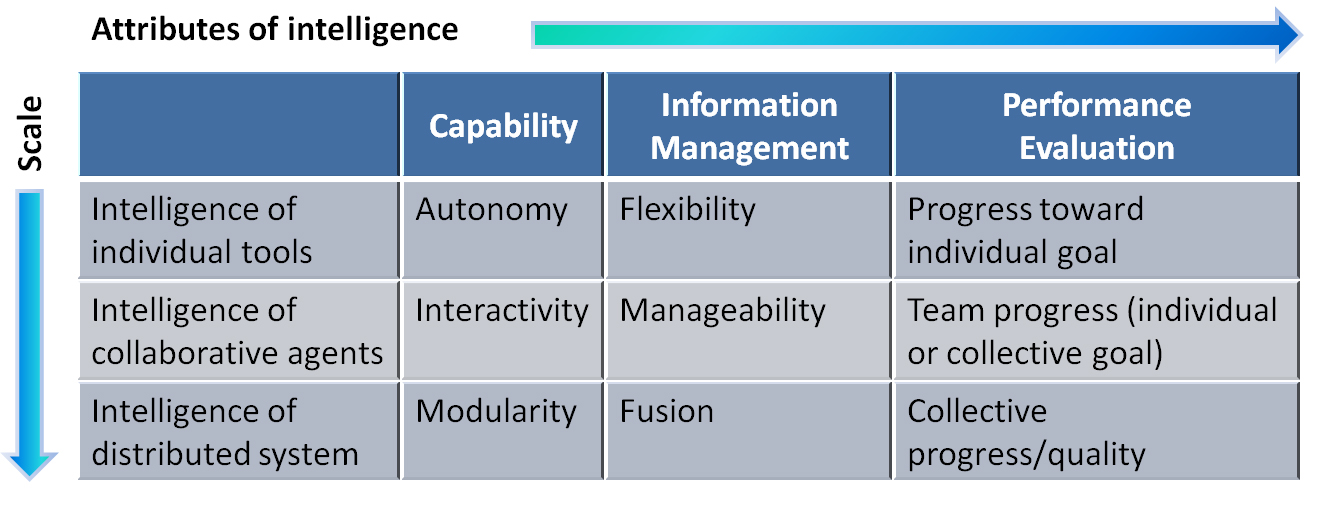
\includegraphics[width=3.5in]{IntegrationChallenges.JPG}
\caption{Autonomy integration challenges defined along two dimensions. Horizontal dimension: attributes of intelligence. Vertical dimension: scale.}
\label{IChallenges}
\end{figure}

%=================================================================================
\section{Autonomy Design Guideline and New Dimensions}
\label{sec:dimensions}

%===================================================
\subsection{Autonomy Design Guideline}

In our previous work~\cite{Lin2010Supporting} we organized the challenges of autonomy and management tool design along two dimensions: \textit{attributes of an intelligent system} (capability, information management, performance evaluation) and \textit{scale} (individual versus group), which can serve as a guideline in designing autonomous components and autonomy management tools. Here we extend this table by adding a row in the middle describing what attributes are needed when multiple agents work collaboratively (see Figure~\ref{IChallenges}). A human-automation team working on the same task falls within this category. As an individual tool, an autonomous component needs to be able to perform a task (\textbf{Autonomy}); the operator can match capability to task according to the information available to the operator, which requires that antonomy can be interrupted, paused, aborted, and resumed (\textbf{Flexibility}); the performance is evaluated to match individual task goal. When a human-automation team works on the same task collaboratively, the autonomous component needs to provide interfaces so the human can influence the autonomous behavior with human inputs (\textbf{Interactivity}); the human agent should be able to manage how autonomy works in order to jointly find a solution by utilizing information only available to the human agent and/or feed information to autonomy in a representation that autonomy can understand (\textbf{Manageability}); and when performance is evaluated, the human operator can judge whether the individual goal aligns with the collective goal of the system. As part of a larger distributed system, each autonomous component needs to be modular (\textbf{Modularity}), so they can be mixed and matched to support different user roles; information from various sources need to be combined and presented to one or multiple users in a \textbf{Fusion}; and performance of the system needs to be evaluated as a whole. This paper focuses on the middle row of this guideline: intelligence of collaborative agents (human-automation team). The three dimensions we propose are ways path planning autonomy can be managed, and the path planner component is designed to accept human inputs along the three dimensions to provide interactivity. The human can also incorporate information from various sources and influence the behavior of path planning autonomy, making sure the task goal aligns with the ultimate goal of finding the missing person quickly.

\begin{figure}
\centering
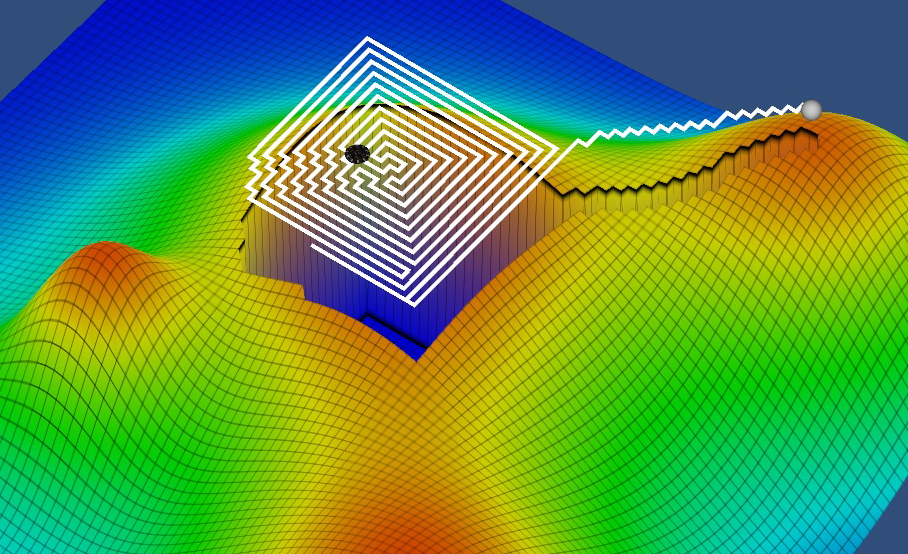
\includegraphics[width=3.5in]{Dimensions.JPG}
\caption{A screen capture of the sliding autonomy tool showing a 20 minute path. The 3D surface shows the probability distribution map. The UAV icon in the middle incidates the start point of the path segment and the sphere on the right indicate the end point.}
\label{dimensions}
\end{figure}

%===================================================
\subsection{Information Representation Dimension}

Many path planning algorithms uses a probability distribution map that shows where are likely places to find the missing person. We also designed our path planning algorithms to support a task-difficulty map: a spatial representation showing (one minus) sensor detection probability in different parts of the search region. For example, probability near the last known position (LKP) of the missing person is normally high; and the probability of detecting the missing person in a dense vegetation area from camera footprints is normally low (high task difficulty). The objective of path planning is to find a path that maximize the detection probability of the missing person given a fixed flying time. The maps can be systematically generated based on terrain features and vegetation data~\cite{Lin2010Bayesian, Lin2014Hierarchical}. However, the searcher likely wants to include his/her domain experties (past experience, knowledge of the search region, etc.) and additional information (maybe new evidence found during the search) in the planning. These types of information are not directly understandable by autonomous algorithms, but the searcher can incorporate them into the probability distribution map and the task-difficulty map using map editing tools\footnote{Such as these tools at http://tech.lannyland.com/demos.html.}, thus influence the behavior of path planning autonomy. Marking an area with high probability, the searcher indirectly tells the UAV to treat the area with high priority; marking an area with high task-difficulty, the UAV might make multiple passes over the area to search more thoroughly. The 3D surface in Figure~\ref{dimensions} shows an exmaple probability distribution map where hills (red) indicate high probability and the flat area (blue) indicates low probability.

By managing information representation, the searcher can quickly figure out how his actions will affect the behavior of autonomy, even though he/she has no idea about how autonomy works behind the scene. Our interface supports autonomy management along this dimension. But we choose to not include it in the current user study (due to the one-hour limit per test subject) and leave the evaluation of it in a separate user study.

%===================================================
\subsection{Task Constraints Dimension}

The searcher can also influence the behavior of path planning autonomy by adding constraints to the problem. Constraints can be the start/end points of the path or no-fly zones~\cite{Clark2013Hierarchical}. Setting an end point in an area is a way for the searcher to indirectly tell path planning autonomy that he/she wants the UAV to search this area. For example, if a piece of clothing is found by the ground team, the seacher can force path planning autonomy to go visit that area by setting an end point there. The searcher can also use this method to direct path planning autonomy to not visit an area by setting the end point in other areas, because that area might have been thoroughly searched by the ground team. By managing autonomy along this dimension, the searcher can incorporate additional information, information not directly understandable by autonomy, to improve task performance and align the task goal with the overall goal of finding the missing person quickly. A no-fly zone is pretty straight foward way to restrict the UAV from visiting certain areas maybe due to safety reasons. In Figure~\ref{dimensions}, the UAV icon in the middle indicates the start point of the path segment and the sphere on the right side indicates the desired end point. Because start/end points and no-fly zones are all spatial constraints, the searcher manages autonomy along a spatial dimension.

Spatial constraints are easy to understand, so the searcher knows how these constraints will affect the behavior of path planning autonomy. In our user study we fixed the start point of the path to the center of the map because that was the last know position of the missing person. The searcher can set the end point for the current path segment anywhere on the map, and this end point automatically becomes the start point for the next path segment. No-fly zone was not tested in our user study.

%===================================================
\subsection{Time Allocation Dimension}

Once the information representation and task constratins (optional) are set, the searcher can use a slider to allocate different time to path planning autonomy. For example, as shown in Figure~\ref{dimensions}, for a 60-minute total flight, the searcher can set an end point to the probability hill on the right, and then move the slider to see immediately what path segment autonomy would suggest. The path segment shown is when 20 minute are allocated. If the searcher is happy with the suggestion, he approves the path segment. The UAV moves to the end point and ``vacuums up'' the probability along the path (how much can be vacuumed up is determined by the task-difficulty map). Then the searcher work together with autonomy to plan the path for the remaining 40 minutes. The two path segments are joined to form the final path. In the example shown, the combination of the information representation, task constraints, and time allocation allows the searcher to cover the middle area pretty well and then move to the search area on the right ready to search there. If no constraint is set, autonomy might decide to search the probability hill on the left instead. If more flight time is allocated with the set end point, autonomy might start searching the area on the right. Because the searcher decides how many path segments to plan and how much time to allocate to each path segment, the searcher manages autonomy along a temporal dimension.

As the search moves the slider to control time allocation, the sliding autonomy tool provides suggested path segment immediately. This instant feedback provides the searcher the ability to perform ``what-if'' analyses and see the causal effect between his/her action and changes in autonomous behavior. 

By managing time allocation, the searcher can break the path planning task into subtasks. The objective of path planning autonomy is to maximize the amount of probability the UAV can collect following the current path segment. The objective of the human or the entire distributed system (where the UAV is only a part of the operation) is to find the missing person quickly. By setting constraints and change the amount of time allocated to a path segment, the searcher has the ability to incorporate additional information into the problem, and align the task goal with the overall system goal. The ability to break the task into subtasks also enables the searcher to plan more strategically (prioritizing areas in the entire search region) while autonomy works more tactically (covering the current search area well). Ideally such a human-automation team should work better than either human or autonomy working alone.


%=================================================================================
\section{Related Work}
\label{sec:RelatedWork6}

Drucker defines automation as a ``concept of the organization of work~\cite{Drucker2006Practice}.'' Goodrich and Schultz~\cite{Goodrich2007HRISurvey} define the HRI problem as ``understanding and shaping the interactions between one or more humans and one or more robots.'' They also specified robot-assisted search and rescue as a key area for HRI research. In their 1978 seminal paper~\cite{Sheridan1978Human}, Sheridan and Verplank propose the idea of a \textit{Level of Autonomy} spectrum, with full teleoperation at one end and full autonomy at the other. In the middle, the robot could suggest actions to humans or make decisions before informing humans. Parasuraman et al.\ \cite{Parasuraman2000Model} extended this one-dimensional spectrum to four different broad functions: information acquisition, analysis, decision selection, and action implementation. In~\cite{Sheridan1992Telerobotics} Sheridan proposes \textit{Supervisory Control}, in which a human divides the task into a sequence of subtasks that the robot is capable of performing, and the human then provides guidance when the autonomous system cannot solve a problem on its own. In contrast to the top-down philosophy of supervisory control, a \textit{Mixed-initiative} approach advocates the idea of dynamically shifting tasks when necessary~\cite{Hearst1999Mixed}. \textit{Collaborative Control}, which can be thought of as an instance of mixed-initiative interaction, is a robot-centric model; instead of the human always being in-charge, the robot is treated as a peer and can make requests to humans through dialogs~\cite{Fong1999Collaborative}. \textit{Adjustable Autonomy}~\cite{Dorais2001Designing} (also referred to as \textit{Sliding Autonomy}~\cite{Dias2008SlidingAutonomy} or \textit{Adaptive Automation}~\cite{Rouse1988Adaptive}) is another type of mixed-initiative interaction, one that enables the human-automation team to dynamically and adaptively allocate functions and tasks among team members. 

Dorais et al.\ \cite{Dorais1998AdjustableAutonomy} discuss a framework for human-centered autonomous systems for a manned Mars mission. The system enables users to interact with these systems at an appropriate level of control but minimize the necessity for such interaction. Bradshaw et al.\ discuss principles and pitfalls of adjustable autonomy and human-centered teamwork, and then present study results on so-called ``work practice modeling'' and human-agent collaboration in space applications~\cite{Bradshaw2003AdjustableAutonomy}. In~\cite{Kaber2005Adaptive} Kaber et al.\ describe an experiment simulating an air traffic control task where manual control was compared to Adaptive Automation (AA). Results suggest that humans perform better with AA applied to sensory and psychomotor information-processing functions than with AA applied to cognitive functions; these results also suggest that AA is superior to completely manual control. Brookshire et al.\ present preliminary results for applying sliding autonomy to a team of robots performing coordinated assembling work to help the system recover from unexpected errors and to thereby increase system efficiency~\cite{Brookshire2004Preliminary}. Dias et al.\ identified six key capabilities that are essential for overcoming challenges in enabling sliding autonomy in peer-to-peer human-robot teams~\cite{Dias2008SlidingAutonomy}. Bradshaw et al.\ \cite{Bradshaw2004Dimensions} propose two dimensions of Adjustable Autonomy (descriptive and prescriptive) to address the two senses of autonomy (self-sufficiency and self-directedness) and discuss how permissions, obligations, possibilities, and capabilities can be adjusted. Bradshaw et al.\ \cite{Bradshaw2013Seven} also summarized some widespread misconceptions on autonomy and listed seven deadly myths of ``autonomous systems.''

Human is an integral part of the human-automation team. When working with automation, the human often takes on the supervisor role. Bainbridge points out that automation requires the human operator to take additional management responsibilities~\cite{Bainbridge1983Ironies}, and Sartar identified in~\cite{Sarter1998Making} two automation management policies: \textit{management by consent} and \textit{management by exception}, defining whether the human always retain authority or can the system take initiative. For complex automations, the human tends to rely on his/her \textit{mental models} (defined by Norman in~\cite{Norman1983Some}) to manage the system. 

UAV technology has emerged as a promising tool in supporting WiSAR~\cite{Murphy2008Cooperative,Bourgault2003Coordinated}. The goal of our research is to support fielded missions in the spirit of Murphy's work~\cite{Casper2003Human}. Many path planning algorithms in the literature address obstacle avoidance while planning a path to reach a destination using A*~\cite{Quigley2005Towards}, LRTA*~\cite{Howlett2006Learning}, D*~\cite{Stentz1997Optimal}, Voroni diagrams~\cite{Bortoff2000Path,Beard2005Autonomous}, or probability roadmaps and rapidly-exploring random tree (RRTs)~\cite{Pettersson2006Probabilistic}. Hierarchical heuristics approaches were also developed, such as Hierarchical A* (HA*) by Holte et al.\ ~\cite{Holte1996Hierarchical}, hierarchical task-based real-time path planning by Naveed et al.\ ~\cite{Meuleau2007Hierarchical}, and Hierarchical-AO* (HiAO*) by Meuleau and Brafman~\cite{Naveed2010Hierarchical}. In~\cite{Bourgault2006Optimal, Bourgault2004Coordinated} Bourgault et al.\ describe how to use a Bayesian model to create paths for a single UAV or multiple coordinated UAVs to maximize the amount of probability accumulated by the UAV sensors. The algorithms we used in this paper are algorithms designed from our previous work~\cite{Lin2009UAV,Lin2014Hierarchical} using techniques such as global warming technique, convolution, Gaussian mixture models, and Evolutionary Algorithm.

%=================================================================================	
\section{Hypotheses} 
\label{sec:Hypotheses}

We performed a user study to evaluate the usefulness with our proposed sliding autonomy approach. More specifically we verify the following hypotheses:

H1: Sliding autonomy method performs better than either the manual path planning method or a semi-autonomous simple pattern path planning method in both low information and high information scenarios.

H2: Sliding autonomy method performs better than autonomy working alone in both low information and high information scenarios.

H3: Sliding autonomy method does not increase the mental workload of the operator.

%=================================================================================	
\section{User Study Design} 
\label{sec:Design}

\begin{figure}
\centering
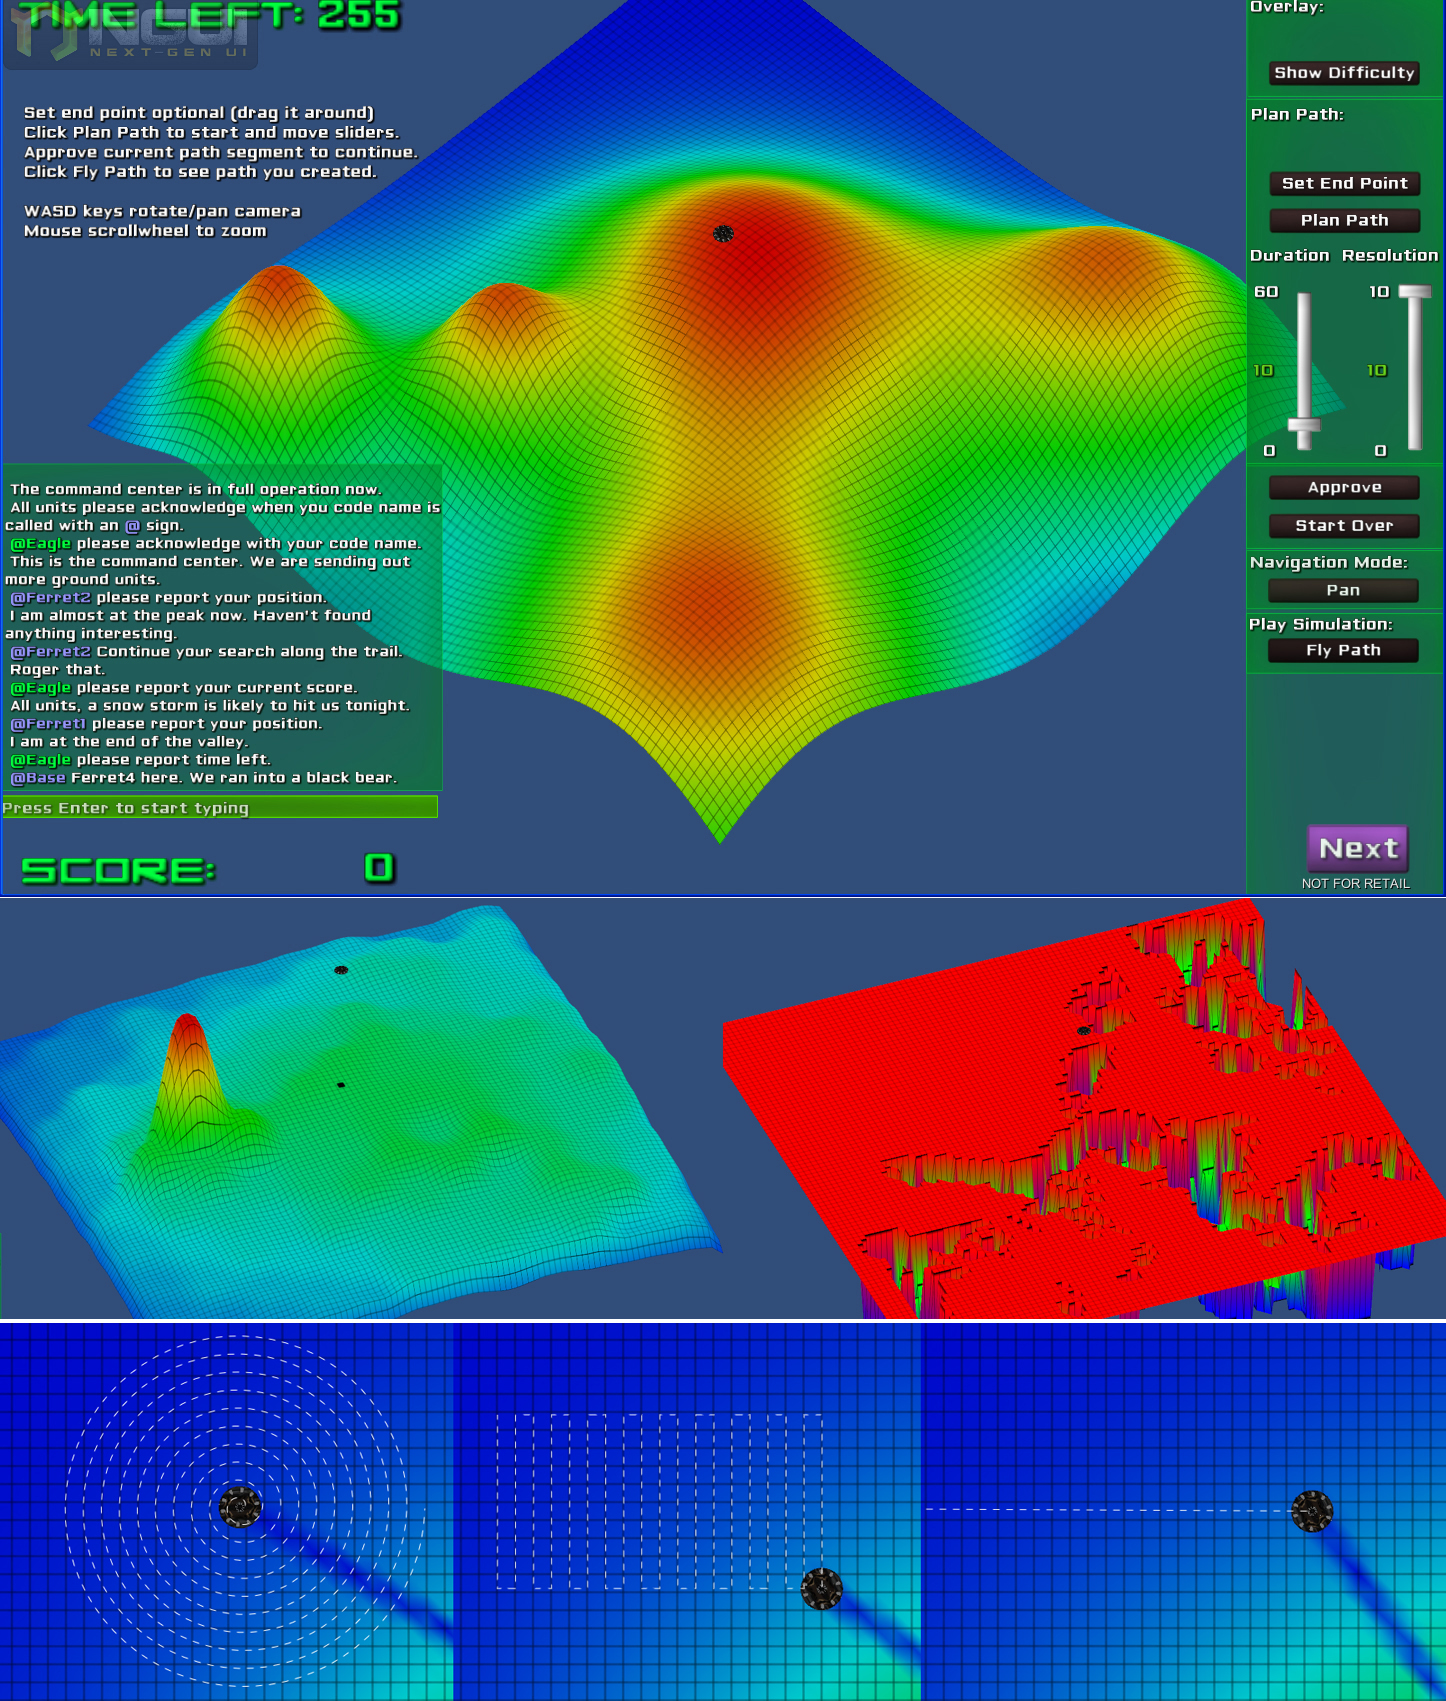
\includegraphics[width=3.5in]{UserStudy.JPG}
\caption{Top: User study simulation interface with sliding autonomy method showing the probability distribution map for scenario 1. Middle left: Probability distribution map for scenario 2. Middle Right: Task-difficulty map for scenario 2. Bottom: The three patterns available to user in pattern planning mode, spiral, lawnmower, and line.}
\label{UserStudy}
\end{figure}

We performed a 2$\times$3 within-subject design with 2 scenarios (easy vs difficult) and 3 planning methods (manual, pattern, and sliding autonomy). All participants completed all 6 exercises. We counterbalanced the order of the scenario and planning methods to reduce learning effect. Half of the participants started with scenario 1, and the order of the planning methods were randomly draw without repeat from the permutation of all possible combinations (without following the same order in both scenarios).

%===================================================
\subsection{Participants}

After analyzing data collected from a pilot study with 6 volunteers, it was dertermined that 25 participants would likely produce significant test results. We recruited a total of 26 college students (14 male males and 12 females) between the age of 19 and 30 (average 23). None has colorblindness. The majority has no experience with robots (57.69\%), and 34.62\% of them are slightly experienced with vacuuming robots.

%===================================================
\subsection{Simulation Environement}

The user study is conducted in a 3D simulation environment. The top portion of Figure~\ref{UserStudy} shows a screen capture of the simulation interface. Both the probability distribution map and the task-difficulty map are displayed as 3D surfaces with a color map (red means high altitude and blue means low) and the user can switch between the two maps anytime. The user can also rotate/pan a map and zoom in/out at will. The UAV in the simulation is a hexacopter that's capable of flying in all directions and hover in the same spot.

With the manual planning method, the user can fly the UAV around with arrow keys as the clock is running in a sped up fassion. The user can freely switch between two flying modes, turn mode and strafe mode, and four camera views, global view (always north up with full view of the map), behind view, bird's eye, and free form view (where the user can rotate/pan/zoom while flying). The user can pause/resume the flight and path planning to perform the secondary task or just review the search area for better planning.

With the pattern planning method, the user can choose from three simple patterns (spiral, lawnmower, and line see the bottom portion of Figure~\ref{UserStudy}) and join these patterns to form the final path. As the user moves the cursor around, the size of the pattern changes with the cursor position marking the end of the path segment (up to the remaining flight time to keep the path valid). Rotation of the lawnmower pattern can be achieved by rotating the map left/right instead. And rotating the map up/down turns the perfect spiral pattern into an ellipse pattern. The user also can undo the last path segment created all the way back to the start.

With the sliding autonomy method, the user can (optionally) set an end point anywhere on the map for the current path segment and then click the \textbf{Plan Path} button to see the path suggested by autonomy.  

Say we did a user study and evaluated these two dimensions with two scenarios. Things we didn't evaluate: no-fly zone, changing maps.
We compared against two planning methods: manual, pattern. Sliding autonomy performed the best.

Human understands manual and pattern.
They don't really know how autonomy works.


%===================================================
\subsection{Scenarios}

Mention real case. Where maps are from.
Scenario 1 no task-difficulty map.

%===================================================
\subsection{Secondary Task}

In~\cite{Vicente1997Should} Vicente suggests to follow the ecological approach~\cite{Rasmussen1994Cognitive} and design interfaces compatible with the actual constraints of the environment so the operator's understanding corresponds to the actual behavior of the system. 


%===================================================
\subsection{Procedure}

0. After signing consent form, fill demographic survey.
1. Training in three modes. Especially manual twice for with task-difficulty map.
2. Has to complete all training, cannot skip.
3. Cheat sheet explaining simulation environment and key concepts.
4. Order of planning modes counter-balanced to eliminate learning effect. Half did scenario 1 first and half did 2 first.
5. Can finish early when use is happy with path (so secondary task is comparable). 5 minutes total for each exercise.
6. After each exercise, NASA TLX.
7. Post user study survey. 

%===================================================
\subsection{Measures}

Primary task: score (comparing against scenario best to normalize, and we pick the best one), time spent, retries, mouse clicks (and mouse clicks/try), NASA TLX
Secondary task: error rate, delay

Compare against LHC alone, and EA, and LHC one input.

%=================================================================================	
\section{Results} 
\label{sec:Results}

With respect to hypotheses:
1. True
2. True
3. True

Sliding autonomy performed significantly better in both senarios.
LHC better than manual and pattern on average.
Sliding autonomy performed better than LHC.
Sliding autonomy performed better than EA in Scenario 1, but not scenario 2.
One input better than EA





69.23\% prefer pattern.
53.85\% thinks manual is easiest to learn. 
57.69\% thinks poattern is easiest to use.
65.38\% thinks sliding autonomy performed the best. (In fact sliding autonomy did best for every one in every scenario).



%=================================================================================	
\section{Discussion} 
\label{sec:Discussion}

Why team performed better?

``Humans, though fallible, are functionally rich in reasoning strategies and their powers of observation, learning, and sensitivity to context.'' ~\cite{Bradshaw2013Seven}

Human is just better at planning at higher abstract level while autonomy is much better at precisely and quickly covering an area (especially with irregular shapes).


\begin{figure}
\centering
\includegraphics[width=3.5in]{placeholder.JPG}
\caption{New dimensions for autonomy management.}
\label{placeholder}
\end{figure}


Why sliding autonomy didn't perform better in secondary task?

David Woods and Eric Hollnagel summarized this phenomenon as the law of stretched systems: ''every system is stretched to operate at tits capacity; as soon as there is some improvement, for example in the form of new technology, it will be exploited to achieve a new intensity and tempo of activity.''  ~\cite{Woods2006Joint}

Difference in planning methods: 
Manual is more physical, but less puzzle solving. People don't get as sucked in, so actually answer more questions. Make up difference.
Pattern and sliding autonomy are like solving puzzles. People get sucked in, and forget about secondary task.
Sliding autnomy has more interaction with algorithms.


Moray~\cite{Moray1999Mental} provides a good summary of how mental models are used and proposes that mental models ``allow operators to think about causal structures and functions in systems which they must control....'' Goodrich and Boer present a case study of Adaptive Cruise Control design and explain how an automobile driver can switch among multiple mental models and use different management strategies~\cite{Goodrich2002Multiple, Goodrich2003Model}. Lee and See propose that because people respond to technology socially, trust guides reliance when unanticipated situations make it impractical or impossible to understand automation~\cite{Lee2004Trust}. Hoffman et al.\ \cite{Hoffman2013Trust} suggests ``active exploration for trusting''(AET) and hope this approach can promote both trust ``calibration'' and appropriate reliance. Moray also points out that the operator's internal model of the environmental and task dynamics can affect how the operator samples information from the environment, and display interfaces should be designed to attract the right amount of attention~\cite{Moray1990Designing}.

People try too hard in putting in too many inputs. Which is probably not necessary.

Manual has higher NASA TLX score because manual planning method is more of a continuous process. Pattern and sliding autonomy easy to stop and resume.

By design, manual has less retries and less mouse clicks.

Scenario 2 is harder.

Trust issue. with ony one end point, autonomy can perform much better. Maybe long term is better. Calibrate trust.

When human sees obvious error, they cannot resist the desire to correct it, then turning into a fight with autonomy, at the cost of increased mental workload, even though the error might have very little value, and the cost of overall bad performance when human wins on that one little thing. They get mentally sucked in the fight. Also when human thinks he/she sees obvious error (when infact autonomy was right).....

Maybe with more complicated scenarios, human would give up because it's not humanly possible to compute things, and just rely on autonomy more?

Test subjects wants immediate feedback when moving the slider even though they were told about possible delays. When slider has delay, they get frustrated and forget about secondary task. Then they click and click and click, ending up with values not desired (which took longer time to correct). This nagatively affected Sliding Autonomy experience.


-- A lot more retries in Pattern and Sliding Autonomy modes.
-- In scenario 2, after covering the only distinct probability hill, many test subjects switched to task difficulty map flew using that map directly.
-- Maybe too optimistic about own performance in pattern?
-- Desire to combine pattern and Sliding Autonomy.
-- Desire to make minor modifications to path after sliding autonomy.

Our information management approach and proposed tools are compatible with these principles because they allow a user to infer causal relationship between user actions and autonomous behavior changes. The user interface designs enable the user to develop mental models of the system that match how the system truly works and thereby improve the human-automation interaction experience.




%=================================================================================	
\section{Conclusions and Future Work} 
\label{sec:Conclusions6}


The \textbf{SlidingAutonomy} interface allows the user to work with automation as a team and affect the behavior of the path planning autonomy by setting constraints and play with different flight duration. The user study we performed is a short-term study where each user only had a short training before using this interface. Because human's trust in autonomy can change over time, it would be interesting to research how the user's trust gets calibrated when the user uses this autonomy management approach for a long period of time. Would the user be able to gradually identify the weaknesses of the path planning autonomy and remedy correctly? Would the user overtrust autonomy and perform worse in the long run? Or would the user undertrust autonomy because autonomy makes obvious mistakes in certain scenarios? In our user study, the two scenarios used are both relatively easy scenarios. When more complicated \textit{probability distribution map} and \textit{task-difficulty map} are used, the benefit of using the \textbf{Sliding Autonomy} interface might be more obvious, and it would interesting to investigate how users would react to that. It is also possible to let the user specify the number of top regions through the \textbf{Sliding Autonomy} interface for the Top2 and TopN algorithms and see how that would affect the human-automation interaction. These questions can only be answered with a long-term user study, which we leave for future work.

At this scale, while the UAV is in the air during mission, as information is collected and processed by the collective search and rescue team, situation arises when the \textit{probability distribution map} and/or the \textit{task-difficulty map} become incorrect. In cases where these two maps cannot be updated in real-time, how can the user use \textbf{SlidingAutonomy} to manage UAV path planning autonomy to address the information change, maybe avoid certain regions or force the UAV to visit certain regions repeatedly, is another interesting research topic. A user study can be performed to evaluate the human-automation interaction experience and the performance of this Sliding Autonomy approach.



%=================================================================================	
\section*{Acknowledgments}

This work was partially supported by 
the National Science Foundation 
%\_\_\_\_\
under grant number 
0534736 
%\_\_\_\_\_
and by a grant from
the Army Research Laboratory.
%\_\_\_\_\.
Any opinions, findings, and conclusions or recommendations expressed in this material are those of the authors and do not necessarily reflect the views of the sponsoring organizations.

%% Use plainnat to work nicely with natbib. 

\bibliographystyle{IEEEtran}
\bibliography{LannyDissertation}


pictures needed:
1. Two scenarios and also task difficulty map for scenario 2
2. Manual mode, pattern mode, sliding autonomy mode
3. 


%Properly evaluate human-robot interaction has always been a challenging problem due to the diversity of team setups, environmental contexts, and tasks involved. Many metrics have been proposed in the literature. Crandall and Goodrich proposed a metric called Neglect Time to measure interaction efficiency~\cite{Crandall2002Principles}. Together with Neglect Time, Olsen and Goodrich later added Task Effectiveness, Robot Attention Demand, Fan Out, and Interaction Effort to the list of Metrics~\cite{Olsen2003Metrics}. Steinfeld and et al.\ suggest some common metrics for standardizing task-oriented human-robot interaction~\cite{Steinfeld2006Common}. In~\cite{Olsen2007Evaluating}, Olsen presents a set of criteria for evaluating new UI systems. Crandall and Cummings propose in~\cite{Crandall2007Ddentifying} a set of metric classes that can predict how many robots should be in the team and the system effectiveness for single-operator controlling multiple robots. We follow guidelines provided in these papers to validate our proposed solution.

%In order to intelligently plan paths for a UAV, it is necessary to understand missing person behaviors and generate a probability distribution of likely places to find the missing person. Many researchers analyzed past WiSAR cases in order to understand missing person behaviors~\cite{Setnicka1980Wilderness,Hill1998Lost,Syrotuck2000Analysis,Heth1998Characteristics,Koester2008Lost}.~\cite{Syrotuck2000Introduction} describes how to use mathematical models to calculate the probability of detection, probability of area and probability of success. He also describes an example search mission. Researchers also looked at systematically utilizing GIS (Geographic Information System) information for search and rescue applications~\cite{Ferguson2008GIS,Soylemez2006Utility}.

%Due to factors such as lighting conditions, dense vegetation, or human observer cognitive workload, even when sensor footprint covers the location of the missing person, probability of detection can be less than 1. In the 1950's, Koopman discussed the uncertainties in the act of detecting hostile submarines with radars and proposed a concept called the instantaneous probability of detection by one glimpse~\cite{Koopman1956Theory}. He presented simple search algorithms and demonstrated how search effort should be distributed given a prior probability distribution of the target and known law of detection when only a limited total amount of search effort (or time) is available~\cite{Koopman1957Theory}. Stone~\cite{Stone1975Theory} presents various search plans with partial detection models using Lagrange multipliers and maximization of Lagrangians in finding stationary target in very basic search problems when no false targets are present. Washburn~\cite{Washburn1981Search} discusses how to construct optimal search paths for different search problems. The author also developed detection models based on radar/sonar and expanded the fundamentals of search theory to include moving targets. More recent work includes~\cite{Niedfeldt2010integrated} where Niedfeldt et al.\ present a UAV path planning algorithm that utilizes probability of detection and maximizes the probability of identifying an object using a N-step lookahead method, and~\cite{Ryan2010particle} where Ryan and Hedrick developed a control formulation for a fixed-wing UAV that minimizes the entropy of an estimate distribution over a receding horizon for searching a moving target over a fixed time horizon. Stone et al.\ used posterior probability maps and successfully located the wreckage of Air France Flight 447~\cite{Stone2011Search}. Metrics such as Koopman's instantaneous probability of detection by one glimpse~\cite{Koopman1956Theory}, ``seeability'' proposed by Morse et al.\ \cite{Morse2010UAV}, and terrain and vegetation information obtained from USGS~\cite{Lin2010Bayesian} can be used to build a task-difficulty map representing probability of detection in different search subregions.

%The UAV technology is an intelligent system with the integration of many component autonomous algorithms and user interfaces. Integration at this level requires tremendous effort. Salas and Fiore~\shortcite{Salas2004Team} provide great insights on challenges across people and machines, and across time and space in distributed teams. Sycara and Lewis~\shortcite{Sycara2002Integrating} also asked the questions: 1) can a software agent perform the task? and 2) can the agent's assistance contribute toward team performance? Tso et al.\ ~\shortcite{Tso1999Multi} identified that integrating a UAV into the search task creates at least two roles: a pilot that controls the UAV and a sensor operator that analyzes the sensor outputs, and lessons from other search-related domains~\cite{Drury2003Awareness} show that multiple roles are required and these roles can be supported by autonomy algorithms and user interface technologies. These findings motivate and guide our research in developing UAV technology to support WiSAR operations.

\end{document}